\section{Results}\label{sec:results}


% \todo[inline]{I think we can summarize the following paragraphs for a few sentences}

In this section, we detail the findings of our study.  We remind the reader that our main goal with this study is to
better understand the strengths and limitations of the \mas for malware detection using the state-of-the-art
test case generation tool (DroidBot). We explore
the results of our research in two datasets: the \sds (102 pairs of apps) and the
\cds (\apps pairs of apps).

%%  and shed light on a few of
%% blindspots that impact the false negative rate. We hypothesize the presence of two blindspots - dynamic call trace from the entry point to a sensitive API, and the differences in the manifest file of repackaged apps. In Section~\ref{sec:Sensitive APIs}, we summarize the results of our study that estimates the performance of the state of the art in mining sandbox approaches. To this end, we reproduce the approach used by DroidBot in their original paper by presenting the divergent sensitive app sets for each app pair in our dataset. We also present details regarding which sensitive APIs are accessed more commonly with malwares. 
%% %We also present the 
%% %sensitive APIs set more injected by repackaged apps, among 162 explored. 
%% %We perform this initial study since it help solve our R1 and served as a reference to solve R2 and R3. \kn{How does this help solve R2 and R3.}

%% The remainder of this section is structured as follows. Section~\ref{sec:traceResults} presents the results of our study analyzing the impact of dynamic call trace on mining sandbox approaches, thereby answering R2. Section~\ref{sec:manifestResults} presents the results of our study analyzing the impact of modified manifest files on sandbox approaches, thereby answering R3. Section~\ref{sec:implications} presents some insights gained from the overall study and their potential implications.

\subsection{Exploratory Data Analysis of Accuracy}

% \subsection{(Accuracy) False negative rate}\label{sec:Sensitive APIs}

{\bf \sds.}
After running the dynamic analysis via DroidBot, our infrastructure produces
a dataset with the sensitive methods that both app versions call during their execution. We consider that a test
generation tool, in our case, DroidBot, builds a sandbox that labels a an app repackaged version
as a malware if there is at least one call to a sensitive method that (a) was observed
while executing the repackaged version of the app and that (b) was not observed while
executing the original version of the same app. 
If the set of sensitive methods that only the repackaged version of an app calls is empty,
we conclude that the sandbox does not label the repackaged version the app as a malware. We triangulate
this information with the outputs of \vt, which might lead to one of the following
situations:

\begin{itemize}
\item {\bf True Positive}. The \mas labels a repackaged version as a malware and, according to
  \vt, at least two \ses label the asset as a malware.
  
\item {\bf True Negative}. The \mas does not label a repackaged version as a malware and,
  according to \vt, at most one \se labels the asset as a malware. 

\item {\bf False Positive}. The \mas labels a repackaged version as a malware and, according to
  \vt, at most one \se labels the asset as a malware.

\item {\bf False Negative}. The \mas does not label a repackaged version as a malware, and
  according to \vt, at least two \ses label the asset as a malware.
\end{itemize}



Considering the small dataset (102) apps, the \mas for malware detection 
classifies a total of 69 repackaged versions as malware (67.64\%).
This result is close to what Bao et al. report. That is, in the
original paper,  the \mas approach using DroidBot classifies 66.66\% of the
repackaged version of the apps as malware~\cite{DBLP:conf/wcre/BaoLL18}.
This result confirms that we were able to reproduce
the findings of the original study using our
infrastructure. 

\tb{1}{We were able to reproduce the results of
  existing research using our infrastructure,
  achieving a malware classification in the
  small dataset close to what has been reported in
  previous studies.}

In the previous studies~\cite{DBLP:conf/wcre/BaoLL18,DBLP:journals/jss/CostaMMSSBNR22},
the authors assume that all repackaged versions contain a
malicious behavior. For this reason, the authors do not
explore accuracy metrics such as Precision, Recall, and
F-measure ($F_1$). As we mentioned, in this paper we take advantage
of \vt to label our dataset and build a ground truth: we only
consider a repackaged version of an app a malware if the results
of our \vt query report that at least two
\se identify a malicious behavior in the asset.
The first row of Table~\ref{tab:accuracy} shows the accuracy of the
vanilla \mas in the \sds.

\begin{table*}[htb]
  \caption{Accuracy of the \mas in both datasets.}
\centering{
  \begin{tabular}{llrrrrrr} \toprule
    Approach       & Dataset & TP   & FP  & FN  & Precision & Recall & $F_1$ \\ \midrule
    \mas           & \sds    & 52   & 17  & 5   & 0.75      & 0.91   & 0.82  \\
    \mas + Traces  & \sds    & 55   & 30  & 2   & 0.64      & 0.96   & 0.77  \\
    \mas           & \cds    & 155  & 191 & 271 & 0.44      & 0.36   & 0.40  \\
    \mas + Traces  & \cds    & 188  & 352 & 238 & 0.34      & 0.44   & 0.38  \\ \bottomrule
  \end{tabular}
  }
  \label{tab:accuracy}
\end{table*}

We also investigate if one could improve the performance of
the \mas using a more elaborated comparison approach.
That is, instead of only comparing the sets of calls to sensitive APIs,
here we also compare the traces from entry points to such a calls. If there is
at least one trace that appears only during the execution of the
test cases in the repackaged version of the app, we
label that version a a malware.

As we already discussed in this section, the vanilla \mas fails
to detect five malware on the \sds (FN column, first row of Table~\ref{tab:accuracy}),
using DroidBot as test case generator tool. When we introduce trace analysis, we reduce the
number of false negatives to two, with the side effect of increasing the
number of false positives from 17 to 30 (see the second row of Table~\ref{tab:accuracy}).
In general, the accuracy ($F_1$) of the \mas using trace analysis drops from 0.82 to 0.77.

%\begin{obs}{1}{}
\tb{2}{Although the use of Trace Analysis reduces the number of
  false negatives (in comparison with the vanilla \mas), it decreases the
  overall accuracy ($F_1$) of the \mas to detect malware,
  from 0.82\% to 0.77\% in the Small Dataset.} 
%\end{obs}


{\bf \cds.}

Surprisingly, when applied to our complete dataset (\apps apps), the \mas
labels a total of 346 repackaged apps as malware (28.76\% of the total number of repackaged
apps)---for which the repackaged version calls at least one additional sensitive API.
Our analysis also reveals a {\bf negative result} related to the accuracy of the approach: here
the accuracy is much lower compared to what we reported for the
\sds (see the third row of Table~\ref{tab:accuracy}), dropping from 0.82 to 0.40 (a reduction of 50\% in terms of $F_1$).
This indicates that, when considering a more representative dataset, the accuracy of the mining sandbox
approach using DroidBot drops significantly. 

%\begin{obs}
\tb{3}{
  The \mas for malware detection
  leads to a substantially lower performance on the
  \cds (1204 pairs of apps),
  dropping the accuracy in 50\% smaller in comparison to
  what we observed in the \sds.}
%\end{obs}

Therefore, the resulting sandbox we generate using
DroidBot suffers from a significantly low accuracy rate when presented with a representative dataset, 
which encouraged us to endorse efforts aimed at identifying potential blindspots with such approaches.
Nonetheless, enriching the \mas with trace analysis also
decreases the overall accuracy in the \cds (even though we reduce the
number of false negatives with trace analysis, the increasing in the
number of false positives negatively impacts the performance of the
approach). This is shown in the fourth row of Table~\ref{tab:accuracy}).

\todo[inline]{Handrick, I reviewed the text until this point.}

\subsection{Assessment Based on \sscore}

Figure~\ref{fig:ss} shows the \sscore distribution
over the two datasets we use in our research
(the small and the complete datasets).
Recall that the \sscore measures how similar the
benign and malicious versions of an app are.
Interesting, the average \sscore of the
small dataset is 0.77 (median of 0.86 and sd of 0.22). Contrasting,
the average \sscore of the complete dataset is
0.61 (median of 0.70 and sd of 0.33).

\begin{figure}
  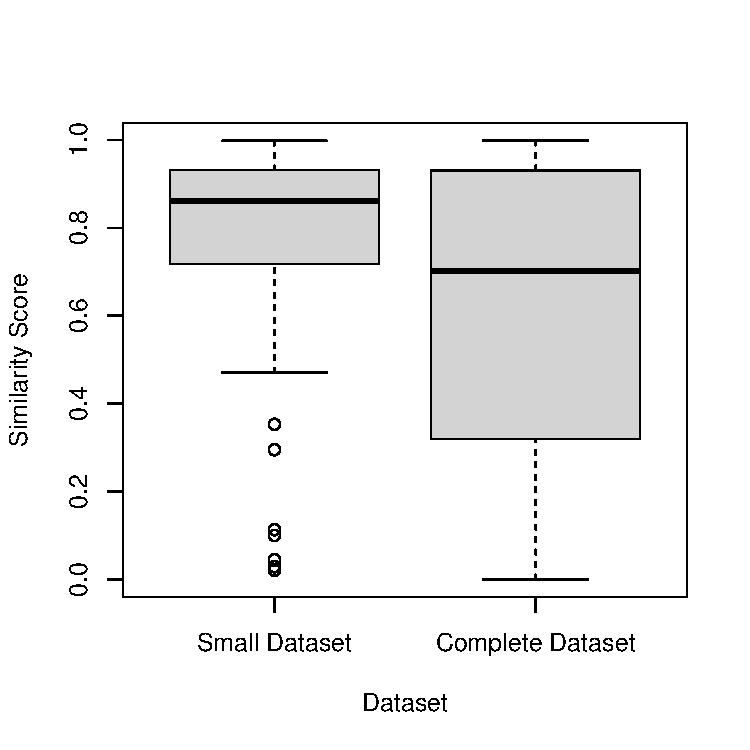
\includegraphics[width=\columnwidth]{images/similarity-1.pdf}
  \caption{\sscore of the malware samples in the small and complete datasets.}
  \label{fig:ss}
\end{figure}

Here we hypothesize that \sscore could explain
the differences of \mas we observed
when comparing the accuracy results for both
datasets. We first use Logistic Regression to test this hypothesis,
and the results reveal
a negative and real association ($p$-value < 0.0005). This find suggests
that repackaged malwares with low similarity with the
original apps are more likely to be identified using the
\mas. This is a contradictory result, since
we found a higher accuracy on the small dataset even though
it presents a higher Similarity
Score on average, in comparison with the complete dataset. 

In a further analysis, we use the \emph{KMeans} algorithm to split the
complete dataset into five clusters, according to the \sscore. We then
estimate the accuracy for each cluster, as
we show in Table~\ref{tab:ss-clusters}. Note that the \mas
achieves the highest accuracy for the samples in the first cluster,
which have an average \sscore of 0.07. Even for this particular
cluster, the \mas achieves an 
accuracy of 37.84\%---still distant from the accuracy
the previous studies report.

\tb{4}{There is a negative and real association between
  the \sscore and the \mas performance. Nonetheless,
  the \sscore does not explain the lower
accuracy of the \mas in the complete dataset.}

\begin{table}[ht]
  \caption{Characteristics of the clusters. Note that the accuracy
  decreases as the average \sscore of the samples in each cluster increases.}
 \centering
 \begin{tabular}{rrrrr}   \toprule
Cluster Id & Sample Size & True Positives & Accuracy & \sscore \\ \midrule
 1 & 190 &  72 & 37.89 & 0.07 \\ 
 2 & 129 &  40 & 31.01 & 0.27 \\ 
 3 & 181 &  60 & 33.15 & 0.51 \\
 4 & 256 &  70 & 27.34 & 0.74 \\ 
 5 & 448 &  99 & 22.10 & 0.94 \\  \bottomrule
 \end{tabular}
 \label{tab:ss-clusters}
 \end{table}
 
\todo[inline]{RB.: I will continue from here tomorrow}

We investigate whether or not the similarity between
the benign and malicious versions of every pair of apps
might explain the accuracy of the \mas for malware detection.

\todo[inline]{I will wait for the new dataset}

---using logistic regression.
The results suggest that we cannot explain the
poor performance of the mining sandbox approach
in terms of the difference between the overall similarity score that occurs in the
complete and small datasets. We also replicate this study using the
malware category feature, though we did not find
statistically significant evidence that the more representative
number of malware categories can explain the lower
performance of the mining sandbox approach in the
complete dataset. 


%% Considering
%% manifest analysis, as we explained in Section~\ref{sec:manifestAnalysis},
%% looking at the occurrence of duplicated permissions and duplicated 
%% components allows us to correctly classify \num{120} out of the \num{607} missed cases
%% from the mining sandbox approach (\num{19.76}\%).                                   
%% Table~\ref{tab:mfa-complete} summarizes the results of this investigation. When considering the 
%% complete dataset (\num{800} apps), combining the vanilla
%% mining sandbox approach (VMS) with trace analysis (TA) and
%% manifest analysis (MA) leads to the correct classification
%% of \num{446} malware (\num{55.75}\%), which suggests that
%% the mining sandbox approach requires further improvements when
%% we take into account a more representative dataset
%% of malware. 


%% \begin{table}[ht]
%%   \centering
%%   \begin{small}
%%   \begin{tabular}{lcc}\toprule
%%   Technique      & Hits & Recall \\ \midrule 
%%   VMS            & 193  & \num{24.12}\% \\ 
%%   VMS + TA       & 369  & \num{46.12}\%  \\
%%   VMS + MA       & 313  & \num{39.12}\% \\
%%   VMS + TA + MA  & 446  & \num{55.75}\% \\  \bottomrule
%%   \end{tabular}
%%   \end{small}
%%     \caption{Summary of the results in the Complete Dataset.}

%%  \label{tab:mfa-complete}
%% \end{table}

%% \begin{obs}{5}{}
%%   The results so far bring evidence that
%%   further research is necessary to understand
%%   the limitations of the mining sandbox approach
%%   targeting more comprehensive datasets.
%% \end{obs}

Our exploration of all sensitive APIs called by all app pairs brought to the light the most frequently abused sensitive APIs that
appear in the repackaged, malicious version of the apps. We observed that when executed all 800 app pairs, DroidBot called $75$ sensitive APIs at least one time (from our list of 162 sensitive APIs). Among them, $16$ APIs account for more than half of all calls ($51.06$\%).
%\rb{I could not understand the previous sentence}.
The sensitive API that is abused the most by repackaged apps is \textbf{android.telephony.TelephonyManager: java.lang.String getDeviceId()}, which gets the device
IMEI\footnote{From Wikipedia: International Mobile Equipment Identity (IMEI) is a number, usually unique, to identify 3GPP and iDEN mobile phones.}.
Table~\ref{tab:APIused} presents the list of the most frequent sensitive APIs that only the malicious
version of the apps in our dataset call.

\begin{obs}{6}{}
  The results so far bring evidence that only a handful of resources accesses like the \textbf{device id} are most attractive to malware designers, providing a potentially high-impact point of focus for future researchers and practitioners.
\end{obs}

%\begin{landscape}
\begin{table*}[t]
 \scriptsize
  \caption{Sensitive APIs more used by repackage apps}
  \centering
  %\begin{small}
 \begin{tabular}{lc}

   \toprule
   Sensitive API & Occurrences \\
   \midrule
   01 android.telephony.TelephonyManager: java.lang.String getDeviceId() &  78 \\
   02 android.net.wifi.WifiManager: android.net.wifi.WifiInfo getConnectionInfo() &  64\\
   03 android.net.wifi.WifiInfo: java.lang.String getMacAddress() &  63 \\
   04 android.net.NetworkInfo: java.lang.String getTypeName() &  58 \\
   05 android.net.NetworkInfo: java.lang.String getExtraInfo() &  56 \\
   06 android.telephony.TelephonyManager: java.lang.String getSubscriberId() &  54 \\
   07 android.net.NetworkInfo: android.net.NetworkInfo State getState() &  52 \\
   08 android.database.sqlite.SQLiteOpenHelper: android.database.sqlite.SQLiteDatabase getWritableDatabase() &  49 \\
   09 android.database.sqlite.SQLiteDatabase: android.database.Cursor query(java.lang.String, ...,java.lang.String) &  47 \\
   10 android.telephony.TelephonyManager: java.lang.String getNetworkOperator() &  45\\
   11 android.telephony.TelephonyManager: android.telephony.CellLocation getCellLocation() &  44\\
   12 android.database.sqlite.SQLiteOpenHelper: android.database.sqlite.SQLiteDatabase getReadableDatabase() &  44\\
   13 android.telephony.gsm.GsmCellLocation: int getLac() &  42 \\
   14 android.telephony.gsm.GsmCellLocation: int getCid() &  42 \\
   
   15 android.net.ConnectivityManager: android.net.NetworkInfo getNetworkInfo(int) &  39 \\
   16 android.telephony.TelephonyManager: java.lang.String getNetworkOperatorName() &  36 \\
   .&  .\\
   .&  .\\
   .&  .\\
   74 android.app.ActivityManager: java.util.List getRecentTasks(int,int) & 1 \\
   75 android.net.NetworkInfo: java.lang.String toString() & 1 \\

 \bottomrule
                            Total & 1592 \\

 \end{tabular}
 %\end{small}
 \label{tab:APIused}
\end{table*}
%\end{landscape}

%% \begin{obs}{1}{}
%%    %\kn{Here we need to add some final take aways of the reproduction study}
%%    Our results indicate that in the presence of a representative dataset ($800$ app pairs as opposed to $102$ and a diverse similarity index), the accuracy of state of the art in mining sandbox approaches, using DroidBot drops significantly (from $63.36\%$ to $24.12\%$). Our results also indicate that only few sensitive APIs are responsible for majority of injected malware in repackaged apps. This encourages the emergence of new proposals that can support mine sandbox mitigating \textit{blindspot}s that lead to low accuracy.
%%  \end{obs}


%\kn{In this subsection, are we simply reproducing the results of existing papers. Because as far as I understand, tools like DroidBOT etc. were evaluated by simply comparing the sensitive APIs call. I am guessing here our contribution is to evaluate it on the larger dataset. I have given it a shot, please keep me posted if this is correct.}

%% \subsection{Trace Analysis Results}\label{sec:traceResults}

%% In this section, we describe the results of our investigation on how the trace from the entry point to sensitive API could impact the accuracy of sandbox approaches. Initially, we collect the call graphs of DroidBot execution using \emph{Logcat} and filter in the traces between the app's entry point and calls to any sensitive methods.

%% Then, using the callgraph from executions of both app versions (benign/malicious), we track the differences between their traces. We choose to investigate only app pairs that covered the same set of sensitive APIs detected in both versions during our first experiment (Section~\ref{sec:Sensitive APIs}). 


%% \begin{obs}{2}{}
%%  The state of the art in mining sandbox approaches using DroidBot have a blind-spot when it comes to being aware of the trace taken from the entry point to a sensitive API call. The approaches could have a improvement of $22\%$ if it considered trace as a factor. Similar  improvements are also seen with the original dataset of $101$ app pairs (improvement of $18.81\%$).
%%  \end{obs}

%% \subsection{Manifest File Analysis}\label{sec:manifestResults}

%% In this section, we describe the results of our investigation on the impact of modified manifest files on the accuracy of sandbox approaches. 
%% To this end, we check some particulars from manifest file, that point to a likely suspicious behavior. In section \ref{sec:manifestAnalysis}, we illustrated that an automatic hacking script could inject permission requests at manifest file regardless of whether this request is already present on it, which can result in duplicated permission and actions in the Manifest file. We looked out for such modifications in the malware that went undetected by the test generation tools. Table~\ref{tab:mfa} summarizes our results.


%% The column (SAPI) indicates the number of malware that went undetected during our first study (same as Table~\ref{tab:pa}'s Same API set (SAPI)). The second column (DP) indicates how many Manifest files from malicious app undetected at first study, had duplicated permission. Same way, column (DA) denotes the number of Manifest files with the duplicated actions in their manifest file.

%% A duplicate request for permission or action in a malicious version's manifest file should have been performed by a script. A simple analysis of manifest file could detect $120$ of undetectable malware from the first experiment ($607$), if it considers explorer duplicate permissions or actions at manifest file code as a detection strategy. If we combine the previous trace analysis with manifest file analysis, we improve the accuracy rate to $55.75\%$.

%% It is to be noted that in the presence of the original dataset of $101$ app pairs, the manifest file analysis combined with the trace analysis earlier discussed improves the accuracy rate to $90.09\%$ confirming that such an analysis, even though naive and simple does have an impact on the accuracy rate of mining sandbox approaches.  %\kn{Handrick as before please put the full numbers in the table}


%% \begin{obs}{3}{}
%%  We can conclude that sandbox approach also could have better accuracy if they considered the suspicious modifications in manifest file in their analysis. Although the analysis required of the manifest file is quite naive, we believe the results present an interesting and relevant insight for developers of malware detection tools to improve accuracy.
%% \end{obs}

%% \todo[inline]{rb: I reviewed the paper until this point. I think that next we should
%% provide more explicit answers to the research questions. kn: Given this a shot}

%% \todo[inline]{mm: any finding we want to formulate related to the discussion in the last paragraph? kn: Given it a shot}

\section{Discussion}

In this section, we explicitly answer our research questions,
summarize the implications of our results, and discuss possible
threats to the validity of the results presented so far.

\subsection{Answers to the Research Questions}

The results we presented in the previous sections
 answer our two research questions, as
we summarize in the following.

\begin{enumerate}[(RQ1)]
\item \textbf{\rqa} 
Our study indicates that the accuracy of the state of the art mining sandbox approaches does not scale.
While the accuracy when applied to a set of approximately $100$ app pairs
was reported to be $66\%$ and confirmed to be $63.26\%$ in our reproduction study, 
it drops to $24.12\%$ in the presence of more representative dataset of $800$ app pairs. 

 \item \textbf{\rqb} Given that considering a combination of trace and manifest analysis improved the accuracy of DroidBot by a factor of $23.34\%$ respectively $31.63\%$ when applied to the small, respectively the complete dataset, it is fair to say that these two hypothesized blindspots do have a significant impact on the accuracy of mining sandbox approaches. 
\end{enumerate}


\subsection{Implications}\label{sec:implications} 

Contrasting to previous research works~\cite{DBLP:conf/wcre/BaoLL18,DBLP:conf/iceccs/LeB0GL18,DBLP:journals/jss/CostaMMSSBNR22},
our results 
%discussed in the previous sections 
lead to a more systematic understanding
of the limitations of using the Android mining sandbox approach
for malware detection. In particular, we show that,
in the presence of a large dataset, the performance of the
approach drops significantly. 

We also highlight that considering only the differences in the
sets of calls to sensitive APIs also leads to false negatives. We
argue in favor of using a more elaborate \emph{diff} approach, which
extends the mining sandbox approach to include the comparisons of
the dynamic call traces from the ``entry points'' of an Android app to its
set of calls to the sensitive APIs. We collect these call traces while
building the sandbox in the usual way~\cite{DBLP:conf/icse/JamrozikSZ16}. Using this extension, we could improve
the performance of the vanilla mining sandbox approach by a factor
between 19\% (small dataset) to 22\% (complete dataset). We
also explored a more ``complementary'' approach, somewhat independent
of the mining sandbox approach, which statically search for two
specific patterns of changes in the Android manifest files: permission
duplication and component duplication. Using the manifest analysis,
we complement the performance of the mining sandbox approach, improving its performance by
a factor between 15\% (complete dataset) and 17\% (small dataset).
Altogether, the implications of this research are twofold:

\begin{description}
  \item[A warning to the community:] the mining sandbox approach for malware detection exhibits a much higher false negative rate  than previous research reported. 
  \item[Future directions:] researchers should advance the mining sandbox approach for malware detection by exploring more advanced techniques for differentiating benign and malicious versions of the apps. 
\end{description}  


